\documentclass[pmlr,twocolumn,10pt]{jmlr} 
\usepackage{graphicx} % Required for inserting images
\usepackage{ifpdf}
\usepackage{cite}
\usepackage{epsfig,graphicx}
\usepackage{float}
% \usepackage[cmex10]{amsmath}
\usepackage{algorithm,algorithmic}
\usepackage{microtype}
\usepackage{amsmath}
\usepackage{mathtools}
\usepackage{amssymb,amsmath,epsfig, graphics,floatflt}
\usepackage{comment}
\pagestyle{empty}
\usepackage{amsmath}
\usepackage{subfigure}
\usepackage{array}
\usepackage{fixltx2e}
\usepackage{subcaption}
\usepackage[labelformat=parens,labelsep=quad,skip=3pt]{caption}
\usepackage{url}
\newlength\myindent
\setlength\myindent{2em}
\newcommand\bindent{%
  \begingroup
  \setlength{\itemindent}{\myindent}
  \addtolength{\algorithmicindent}{\myindent}
}
\newcommand\eindent{\endgroup}

\begin{document}
%\title{Narcondam Hornbill Algorithm - An Algorithm for Automated and Efficient Seed Dispersal in Barren Lands}
\title{A Novel Narcondam Hornbill-based Seed Dispersal in Barren Lands}
\author{BEERELLY SRINITHA and SIKANDER KATHAT}
%\date{February 2023}

\maketitle

%%%%%%%%%%%
%Abstract: Write two lines about why you want to do this work, and the challenges or issues involved in it, to solve these issues we are proposing the algorithm ...., this algorithm is tested and implemented.....
%%%%%%%%%%%%%
\section*{Abstract}
Seed dispersal plays a crucial role in the survival of plant species, but human activities are disrupting this process, leading to ecosystem degradation. There is a need to develop innovative seed dispersal algorithms to restore degraded ecosystems and prevent further biodiversity loss. Drones can be used as powerful tools to assess the state of ecosystems, identify areas requiring seed dispersal, and monitor restoration progress. By leveraging drones, more effective seed dispersal algorithms can be developed to promote diverse plant communities and ensure long-term ecosystem sustainability. One of the challenges in simulating seed dispersal is the difficulty in accounting for the complex interactions between different environmental factors and seed characteristics. The proposed algorithm aims to address the limitations of existing models and improve the effectiveness of seed dispersal efforts. This algorithm utilizes the endozoochory process of the Narcondam Hornbill to optimize seed dispersal efficiency, which has been successfully tested and implemented in simulated environments.
\section{Introduction}
Seed dispersal is a crucial process that contributes to the survival and diversity of plant species. In nature, seed dispersal is carried out by a variety of mechanisms such as wind, water, animals, and birds. Among these, avian seed dispersal, or ornithochory, is considered to be one of the most effective methods for seed distribution, as birds can cover large areas quickly and disperse seeds over a range of habitats. 
\\The efficient and effective dispersal of seeds is essential for the survival and regeneration of many plant species, but anthropogenic factors are increasingly disrupting this process, leading to biodiversity loss and ecosystem decline. In the absence of scalable and practical solutions, up to 95\% of the world's ecosystems could be impacted by seed dispersal degradation by 2050. Therefore, there is an urgent need to develop and implement innovative seed dispersal algorithms to restore degraded ecosystems and stem biodiversity loss. To achieve this, the most advanced and efficient tools are required, which include unmanned aerial vehicles, or drones. 
\\Drones have proven to be valuable tools in various sectors, such as environmental conservation, forestry, and agriculture. However, their use in restoration ecology for seed dispersal has been limited so far. Therefore, this article aims to highlight the potential uses of drones in seed dispersal algorithms for ecological restoration. Drones can accurately assess the state of ecosystems, identify areas that require seed dispersal and monitor the progress of the restoration process over time. With the help of drones, more effective seed dispersal algorithms can be developed to promote the growth of diverse plant communities and ensure the long-term sustainability of ecosystems.
\\In recent years, computer scientists have developed various algorithms for simulating seed dispersal and optimizing the process for real-world applications. However, many of these algorithms are limited in their efficiency and accuracy and do not fully capture the complexity of the natural processes of seed dispersal.
\\The Narcondam Hornbill can serve as an important source of inspiration for developing more effective seed dispersal algorithms and highlights the potential of avian seed dispersal for restoring and maintaining biodiversity in natural ecosystems. This contributes to the growing body of knowledge on the role of birds in ecosystem functioning and emphasizes the need for innovative and sustainable solutions to address the global challenge of seed dispersal in barren lands.
\\A new seed dispersal algorithm inspired by the endozoochory process of the Narcondam Hornbill is presented. The Narcondam Hornbill is a bird found only on the remote island of Narcondam in the Andaman and Nicobar archipelago and plays a critical role in the seed dispersal of many plant species. By consuming fruits and seeds, the bird helps to transport them to new locations, where they can germinate and grow. 
\\The algorithm is designed to simulate the endozoochory process of the Narcondam Hornbill and to optimize seed dispersal for real-world applications. The various components of the algorithm, including the selection of suitable plant species, the design of the seed mixture, and the simulation of bird movement patterns are discussed.
\section{Narcondam Hornbill}
The Narcondam Hornbill (Rhyticeros narcondami) is a bird species found only on the small island of Narcondam in the Andaman and Nicobar archipelago of India. It plays an important role in seed dispersal on the island.
\\The Narcondam Hornbill feeds on a variety of fruits, including figs, guavas, and other fleshy fruits. As the bird consumes the fruit, the seeds pass through its digestive system and are deposited in its droppings in different locations across the island.
\\This process of seed dispersal through ingestion by birds is called endozoochory. The seeds in the hornbill's droppings have a better chance of germination and growth because they have been partially digested and their hard outer shells have been broken down, making it easier for the young plant to emerge.
\\Overall, the Narcondam Hornbill is an important part of the island's ecosystem, helping to disperse the seeds of many plant species and contributing to the island's biodiversity.
\\However, the Narcondam Hornbill is currently classified as a vulnerable species due to habitat loss and fragmentation, making it increasingly important to study and understand its role in seed dispersal.
\\Furthermore, seed dispersal is a crucial process for maintaining and enhancing biodiversity in natural ecosystems. It allows for plant species to colonize new areas, increase genetic diversity, and support the survival of other organisms. Therefore, developing effective seed dispersal algorithms that can simulate and optimize the process is important for restoration and conservation efforts.
\\Several existing seed dispersal algorithms have been developed, but many are limited in their accuracy and efficiency. As a result, there is a need to explore and develop new algorithms inspired by the natural processes of seed dispersal. The Narcondam Hornbill, with its unique role in endozoochory, provides a valuable source of inspiration for such algorithms.

\section{Proposed Narcondam Hornbill System Architecture}

In this section, we discuss the architecture,stages of seed dispersal, and drone dispatching mechanism.
\subsection{Architecture}

\begin{figure}[htp]
    \centering
    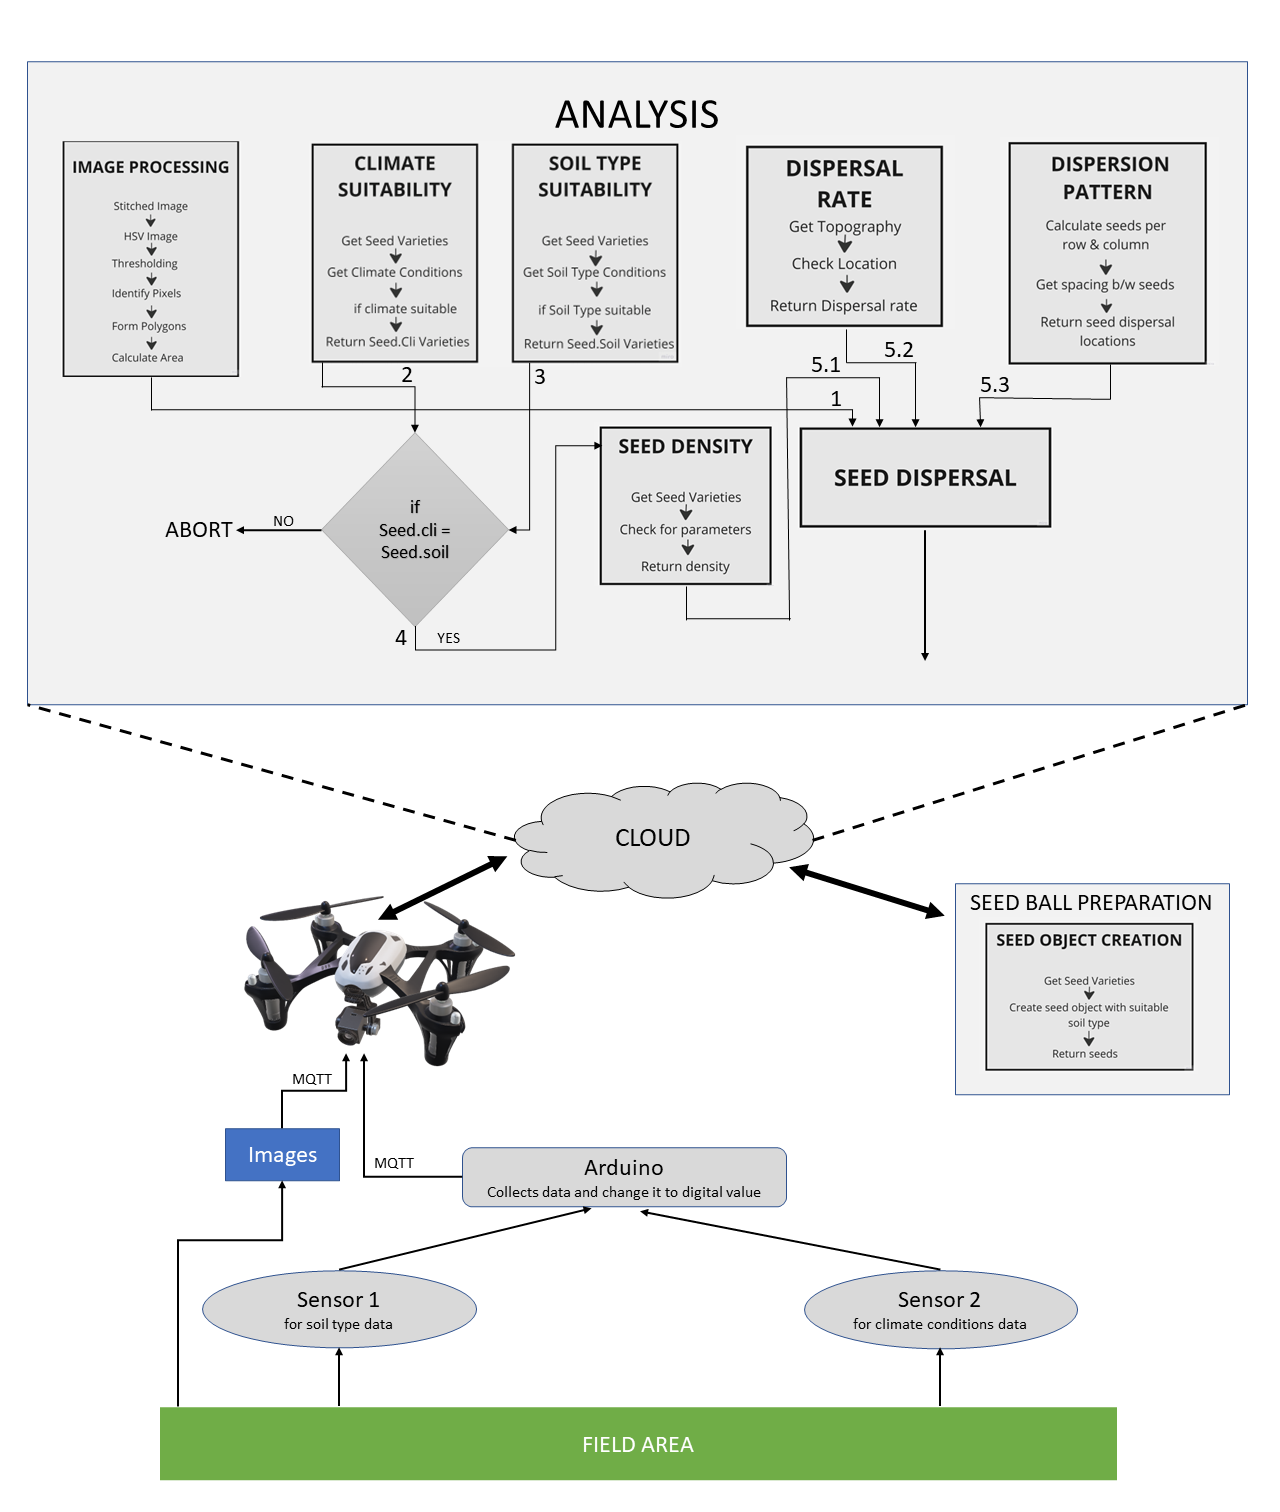
\includegraphics[width=8cm,height=8cm]{architecture_ml.png}
    \caption{SYSTEM ARCHITECTURE}
    \label{fig:galaxy}
\end{figure}

The architecture for this algorithm can be divided into different modules or stages, each of which performs a specific task. Here's a proposed architecture for the algorithm:

\textbf{Image Processing Module:} This module takes the list of captured images as input, stitches them together into a single image, and converts the image to the HSV color space. It then applies a color threshold to identify pixels within the range of barren land color and then it forms a polygon with pixels identified and calculates the total area of the polygon formed of barren land.

\textbf{Climate and Soil Suitability Module:} This module checks if the climate conditions and soil type are suitable for the selected seed variety. It returns a message indicating whether the climate and soil type is suitable or not.

\textbf{Seed Density Module:} This module takes the climate conditions, topography, soil type, and seed variety as input and looks up the recommended seed density for the given seed variety based on the current growing conditions. It returns the recommended seed density as the optimal number of seeds per unit area.

\textbf{Dispersion Pattern Module:} This module takes in the location where the seeds need to be dispersed and the total number of seeds as input. It determines the number of seeds to place in each row and column, determines the spacing between each seed, and returns a list of tuples containing the location of each seed along with its associated seed.

\textbf{Seed Object Creation Module:} This module takes in the soil type and seed variety as input, creates a seed object with the necessary properties such as water level, nutrient level, etc., and returns the seed object.

\textbf{Seed Dispersal Rate Module:} This module takes in the topography and location as input, determines the optimal seed dispersal rate of seeds based on the topography and location, and returns the dispersal rate.

\textbf{Seed Dispersal Module:} This module dispatches the drone to the location and begins seed dispersal. It checks whether the seed dispersal was successful or not and returns a message indicating the success or failure of the seed dispersal.

The above architecture can be implemented using various programming languages and frameworks such as Python, OpenCV, NumPy, etc. Each module can be implemented as a separate function or class, and the overall algorithm can be designed as a series of function calls.

\subsection{Stages of Seed Dispersal}

 A sophisticated and effective seed dispersal strategy contains the following stages of seed dispersal:
 
\textbf{Aerial Survey \& Mapping:} Drones are used to survey and map the terrain to identify places needing plantation. We use hyper-spectral image technology with Machine learning to generate a topographical map to give a holistic sense of the total area.

\textbf{Understanding The Requirements:} Determine trees to be grown based on various parameters like weather, altitude, soil, indigenous seed varieties, and historical growth data using previous information and machine learning.

\textbf{Seed Balls Preparation:} Seed balls are then created as per local soil requirements and in order to ensure safety and no change of direction by the wind.

\textbf{Drone Deployment:} Drones are deployed to spray seeds over designated areas. We fly the drones along a pre-determined flight map. These maps are digitally rendered to cover all the areas determined in Step 1 with a topographical overlay for easy visualization.

\textbf{Geo-tagging Drone path:} The paths followed by the drones are geo-tagged, facilitating periodic drone monitoring of the sown area to collect tree statistics.

\textbf{Post Growth Monitoring:} Geo-tagged seed balls are monitored for growth for years to come to create analytics required for forest monitoring.

\begin{figure}[htp]
    \centering
    \includegraphics[width=8cm,height=8cm]{ML PROJECT FLOWCHART .png}
    \caption{STAGES OF SEED DISPERSAL}
    \label{fig:galaxy}
\end{figure}

\subsection{Dispatching mechanism}

Seed dispersal by drones typically involves using a variety of dispatching mechanisms to release and distribute seeds in a target area. Some possible dispatching mechanisms for seed dispersal by drones include: Drop mechanism, Spray mechanism, Pneumatic mechanism, and Glue mechanism.
\\In addition to these mechanisms, drones may also be equipped with sensors and software to help guide seed distribution and optimize the dispersal pattern. For example, drones may use GPS technology to accurately target specific areas or avoid sensitive habitats, or use machine learning algorithms to adapt to changing wind conditions or terrain.
\\Drop mechanism is used in this study. Seed dispersal by drones using the dropping mechanism involves releasing the seeds from a container mounted on the drone at a specific location. The container may have a small opening or be designed to open automatically when triggered by the drone's software. The drone may hover or fly over the target area and drop the seeds in a pattern determined by the operator or software. The drone may move or rotate as needed to ensure that the seeds are distributed evenly.
\\One advantage of the dropping mechanism is that it can be used to target specific areas with greater accuracy than other dispersal methods. The operator can control the height and speed of the drone to ensure that the seeds are dropped in the desired location. Additionally, the dropping mechanism can be used to release a wide variety of seed sizes and shapes, making it a versatile option for seed dispersal by drones.
\\Overall, seed dispersal by drones using the drop mechanism is a precise and efficient method that can be used to target specific areas with accuracy.
\begin{figure}[htp]
    \centering
    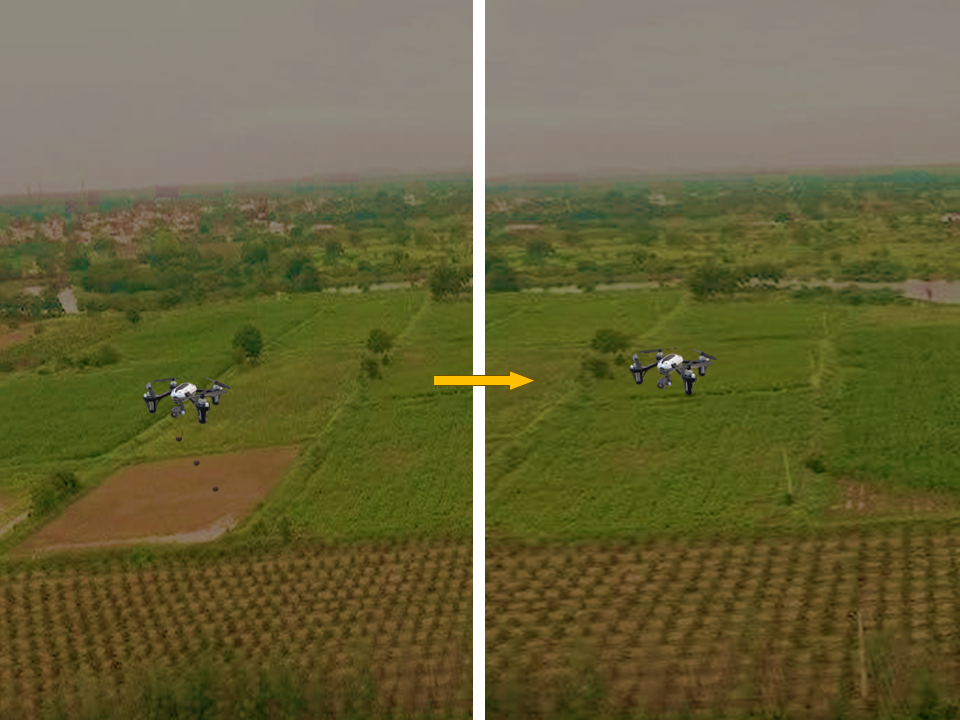
\includegraphics[width=7.5 cm,height=8cm]{Slide2.PNG}
    \caption{DRONE DISPATCHING SEEDS}
    \label{fig:galaxy}
\end{figure}

\section{Narcondam Hornbill Algorithm }

\begin{algorithm} [ht]
\begin{scriptsize}
\begin{algorithmic}[1]

% \STATE Begin
\STATE \textbf{AIM: Declaring functions which will be called in the main function}
\medbreak
\STATE \textbf{find\_barren\_land\_and\_its\_area}(images) 
    \begin{ALC@g}
    \STATE  Stitched\_image $\gets$ stitch(images)
    \STATE  hsv\_image $\gets$ Stitched\_image
    \STATE  Threshold\_image $\gets$ inRange(hsv\_image, lower\_barren, upper\_barren)
    \STATE  contours $\gets$ findContours(Threshold\_image)
    \FOR{contour in contours}
        \STATE  polygon $\gets$ approxPoly(contour, arcLength)
        \STATE  polygons.append(polygon)
    \ENDFOR
    \STATE  area $\gets$ 0
    \FOR{polygon in polygons}
    \STATE  area $\gets$ area + contourArea(polygon)
    \ENDFOR
    \STATE  \Return area
    \end{ALC@g}
\smallbreak
\STATE \textbf{is\_climate\_suitable}(climate, seed\_variety)
    \begin{ALC@g}
    \STATE Suitable\_climate $\gets$ read.dataset[]
    \STATE climate\_Suitable$\gets$Suitable\_climate.get(seed\_variety)
    \IF{climate in climate\_Suitable}
        \STATE \Return True
    \ELSE
        \STATE \Return False
    \ENDIF
    \end{ALC@g}
\smallbreak
\STATE \textbf{is\_soil\_type\_suitable}(soil\_type, seed\_variety)
    \begin{ALC@g}
    \STATE suitable\_soil\_types $\gets$ read.dataset[]
    \STATE Suitable\_types$\gets$suitable\_soil\_types.get(seed\_variety)
    \IF{soil\_type in Suitable\_types}
        \STATE \Return True
    \ELSE
        \STATE \Return False
    \ENDIF
    \end{ALC@g}
\smallbreak

\STATE \textbf{get\_optimal\_seeds\_per\_unit\_area}(climate,topography,\\soil\_type,seed\_variety) 
    \begin{ALC@g}
    \STATE  density$\gets$Suitable\_densities.get(seed\_variety,climate,\\topography,soil\_type)
    \STATE\Return density
    \end{ALC@g}
\smallbreak

\STATE\textbf{disperse\_seeds}(location, total\_seeds)
    \begin{ALC@g}
    \FOR{$i$ \textbf{in range}($seeds\_per\_row$)}
        \FOR{$j$ \textbf{in range}($seeds\_per\_col$)}
            \STATE $x \gets get.disperse\_point\_x(init\_loc, x\_spacing)$
            \STATE $y \gets get.disperse\_point\_y(init\_loc, y\_spacing)$
            \STATE $seed \gets create\_seed('default')$
            \STATE $seeds.append((x, y, seed))$
        \ENDFOR
    \ENDFOR
    \STATE \Return $seeds$
    \end{ALC@g}
\smallbreak
\STATE\textbf{create\_seed}(soil\_type, seed\_variety)
    \begin{ALC@g}
    \STATE \Return $seed$
    \end{ALC@g}
\smallbreak

\STATE\textbf{determine\_dispersal\_rate}(topography, location)
    \begin{ALC@g}
    \STATE \Return $dispersal\_rate$
    \end{ALC@g}
\smallbreak

\STATE\textbf{dispatch\_drone}(location, dispersal\_rate)
    \begin{ALC@g}
    \STATE $drone.takeoff()$
    \STATE $seeds\_dispensed \gets 0$
    \WHILE{$seeds\_dispensed < dispersal\_rate$}
        \STATE $seeds\_dispensed += drone.dispense\_seed()$
    \ENDWHILE
    \STATE $drone.land()$
    \end{ALC@g}


    
\end{algorithmic}
\caption{Narcondam Hornbill Algorithm}
\end{scriptsize}
\label{algo:resuti}
\end{algorithm}


\begin{algorithm} [ht]
\begin{scriptsize}
\begin{algorithmic}[1]
\STATE \textbf{INPUT}:$A$ $set$ $of$ $images$ $of$ $an$ $area$.
\STATE \textit{\textbf{Training data}}: $dataset$ $for$ $climate$ $type,$ $soil$ $type,$ $seed$ $variety$ $and$ $topography.$
\STATE \textit{\textbf{Testing data}}: $A$ $set$ $of$ $images$ $of$ $field$ $area.$
\STATE \textbf{OUTPUT}: $Whether$ $seeds$ $are$ $dispersed$ $or$ $not.$ 
\medbreak

\STATE \textbf{seed\_dispersal}
(images, climate, topography,\\soil\_type,seed\_variety, location) 
    \begin{ALC@g}
    \STATE {is\_climate\_suitable}(climate, seed\_variety)
    \STATE {is\_soil\_type\_suitable}(soil\_type, seed\_variety)
    \STATE  seeds\_per\_unit\_area $\gets$ {get\_optimal\_seeds\_per\_unit\_area}\\(climate,topography,soil\_type,seed\_variety)
    \STATE  area $\gets$ {find\_barren\_land\_and\_its\_area}(images)
    \STATE  total\_seeds = area*seeds\_per\_unit\_area
    \STATE{disperse\_seeds}(location, total\_seeds)
    \STATE  seed\_dispersal\_location.append(location)
    \STATE  success = {dispatch\_drone}(location, dispersal\_rate)
    \IF{(success)}
        \STATE \Return "seed dispersal successful".
    \ELSE
        \STATE \Return "seed dispersal failed".
    \ENDIF
    \end{ALC@g}
    
\end{algorithmic}
\caption{Main Function}
\end{scriptsize}
\label{algo:resuti}
\end{algorithm}

 This algorithm takes in a list of images which are captured by the drone during the aerial survey as input, stitches them together into a single image, converts the image to the HSV color space, applies a color threshold to identify pixels within the range of barren land color, and then calculates the total area of the barren land in the image and returns the area of the barren land as output.
 \\The algorithm then starts checking if the climate conditions are suitable for the selected seed variety. If the climate is suitable, the algorithm returns a message indicating that the climate is suitable for the selected seed variety. The algorithm also checks if the soil type is appropriate for the selected seed variety. If the soil type is suitable, the algorithm returns a message indicating that the soil type is suitable for the selected seed variety.
\\Next, the algorithm takes in the climate conditions, topography, soil type, and seed variety as input looks up the recommended seed density for the given seed variety based on the current growing conditions, and returns the recommended seed density as the optimal number of seeds per unit area. 
\\The algorithm then takes in the location where the seeds need to be dispersed and the total number of seeds as input, determines the number of seeds to place in each row and column, determines the spacing between each seed, creates a seed object, and returns a list of tuples containing the location of each seed along with its associated seed object. 
\\The algorithm then takes in the soil type and seed variety as input creates a seed object with the necessary properties such as water level, nutrient level, etc, and returns the seed object. The algorithm takes in the topography and location as input, determines the optimal seed dispersal rate of seeds based on the topography and location, and returns the dispersal rate. The drone is then dispatched to the location and begins seed dispersal. If the seed dispersal is successful, the algorithm returns a message indicating that the seed dispersal was successful. If the seed dispersal is not successful, the algorithm returns a message indicating that the seed dispersal failed.

\section{Environment Setup}

\begin{figure}[htp]
    \centering
    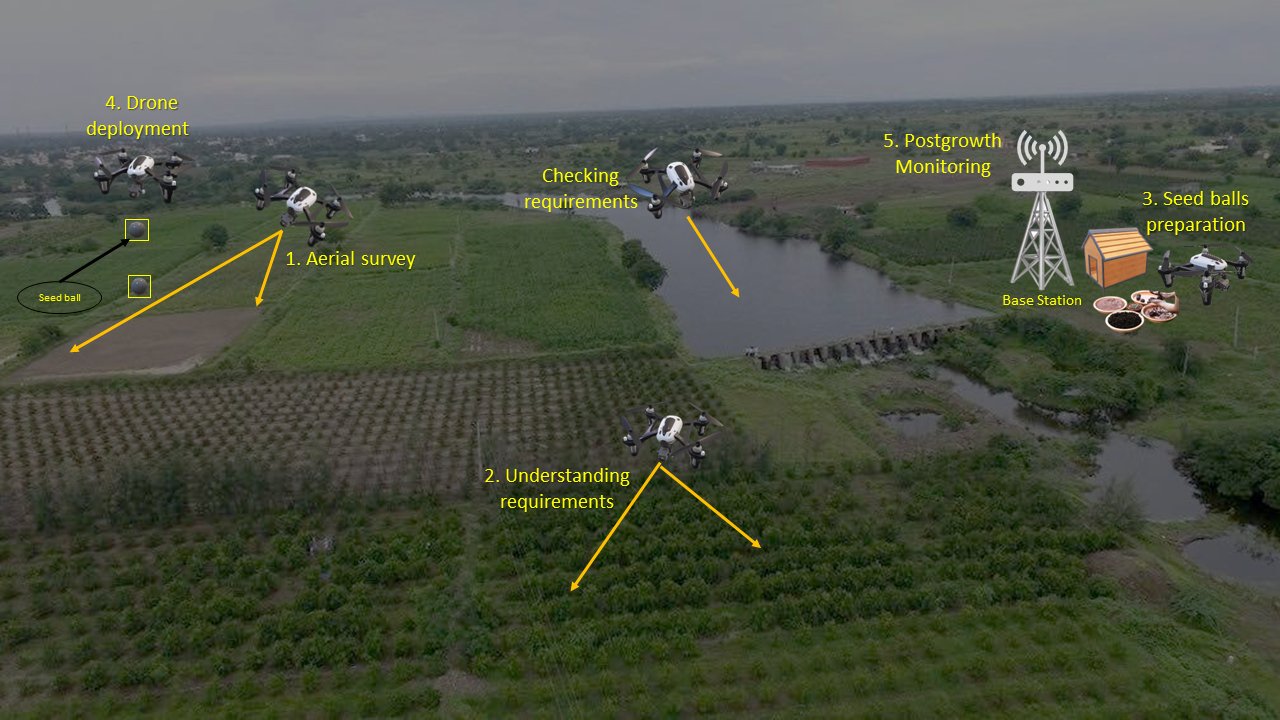
\includegraphics[width=8cm,height=8cm]{hornbill.png}
    \caption{Environment setup map}
    \label{fig:galaxy}
\end{figure}

The above environment setup would be the perfect setup for the experiment and testing. When an unknown environment is given the drone uses our algorithm and performs the seed dispersal. All the stages of seed dispersal are executed one after the other and tested on the given environment.


\section{Simulation and Results Analysis}
In this section, we discuss the simulation scenario, dataset, and results analysis.

\begin{figure}[htp]
    \centering
    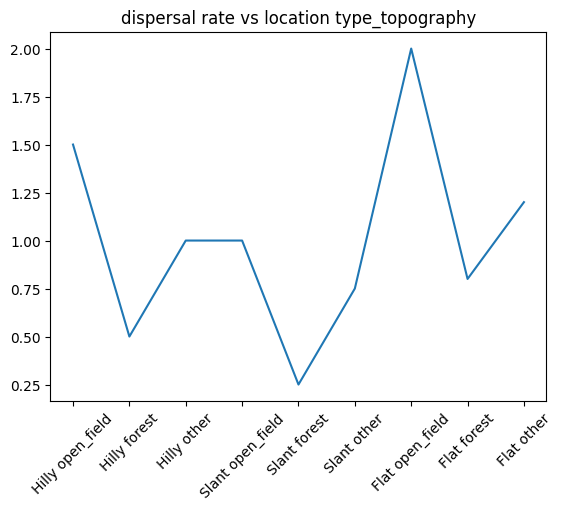
\includegraphics[width=7cm,height=8cm]{download (1).png}
    \caption{Seed dispersal rate with respect to topography}
    \label{fig:galaxy}
\end{figure}

\begin{figure}[htp]
    \centering
    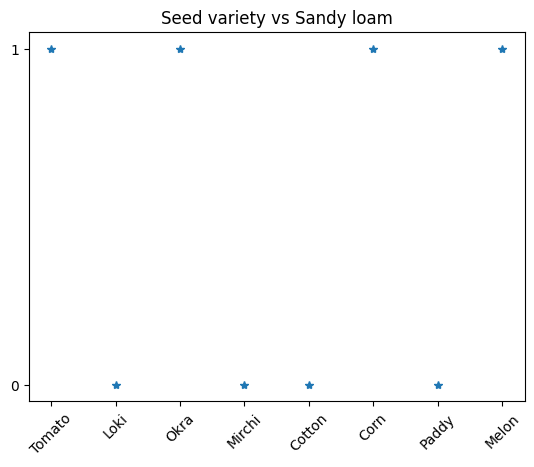
\includegraphics[width=7cm,height=8cm]{download (2).png}
    \caption{Seed variety with respect to sandy loam}
    \label{fig:galaxy}
\end{figure}

\begin{figure}[htp]
    \centering
    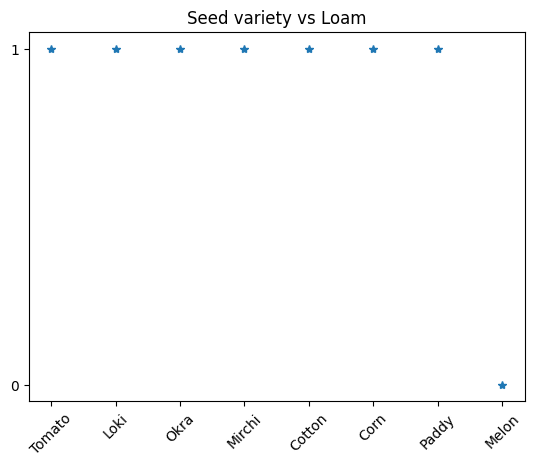
\includegraphics[width=7cm,height=8cm]{download (3).png}
    \caption{Seed variety with respect to loam}
    \label{fig:galaxy}
\end{figure}

\begin{figure}[htp]
    \centering
    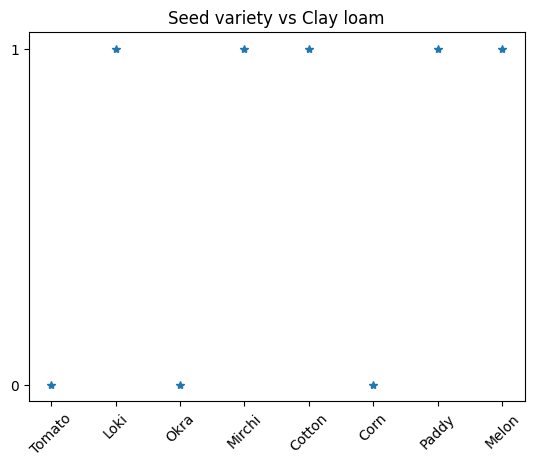
\includegraphics[width=7cm,height=8cm]{download (4).png}
    \caption{Seed variety with respect to clay loam}
    \label{fig:galaxy}
\end{figure}


\section{Conclusions and Future Work}
In conclusion, the Narcondam Hornbill-inspired seed dispersal algorithm provides a novel approach by simulation of the hornbill's dispersal process and its consideration of environmental factors improves the accuracy and efficiency of the seed dispersal process, improving seed dispersal efficiency and accuracy. The algorithm's ability to optimize the process for different environmental conditions and seed types could have significant benefits for plant species survival and ecosystem biodiversity. The algorithm has the potential to greatly improve the effectiveness of seed dispersal in barren lands and may help to mitigate the effects of environmental degradation. The algorithm offers a more efficient and accurate way of simulating seed dispersal in a simulated environment. 
\\In future, the algorithm could be further refined and tested in real-world applications such as reforestation and conservation efforts.

\section*{References}
[1] History of U.S. Drones, Understanding Empire,2016, Available at: https://understandingempire.wordpress.com/2-0-a-brief-history-of-u-s-drones/.
\newline
\newline
[2] Gandham Venkata Sai Lohit; Divyansh Bisht,2021, "Seed Dispenser using Drones and Deep Learning Techniques for Reforestation"
\newline
\newline
[3]Ben Anthony Horton  with Reuters(2022), "These seed-firing drones are planting 40,000 trees every day to fight deforestation"
\newline
\newline
[4] Nishar, A.; Richards, S.; Breen, D.; Robertson, J.; Breen, B. Thermal infrared imaging of geothermal environments and by an unmanned aerial vehicle (UAV): A case study of the Wairakei – Tauhara geothermal field, Taupo, New Zealand. Renew. Energy 2016, 86, 1256–1264.
\newline
\newline
[5] Naniwadekar, R. S. (2020). Narcondam Hornbill (Rhyticeros narcondami), version 2.0. In Birds of the World (S. M. Billerman and B. K. Keeney, Editors). 
https://doi.org/10.2173/bow.narhor1.02
\newline
\newline
[6] BirdLife International. (2021). Species factsheet: Narcondam Hornbill Aceros narcondami. Retrieved from https://www.birdlife.org/
\newline
\newline
[7] Manchi S. S. 2017. Status, Ecology and Conservation of Narcondam hornbill Aceros narcondami on Narcondam island, India (Report No. 189). Salim Ali Centre for Ornithology and Natural History project/Technical consultancy reports. Salim Ali Centre for Ornithology and Natural History. Available at: http://www.sacon.in/publications/reports/.
\newline
\newline

\end{document}




